\documentclass{standalone}
\usepackage{tikz}
\usetikzlibrary{patterns, positioning}

\begin{document}
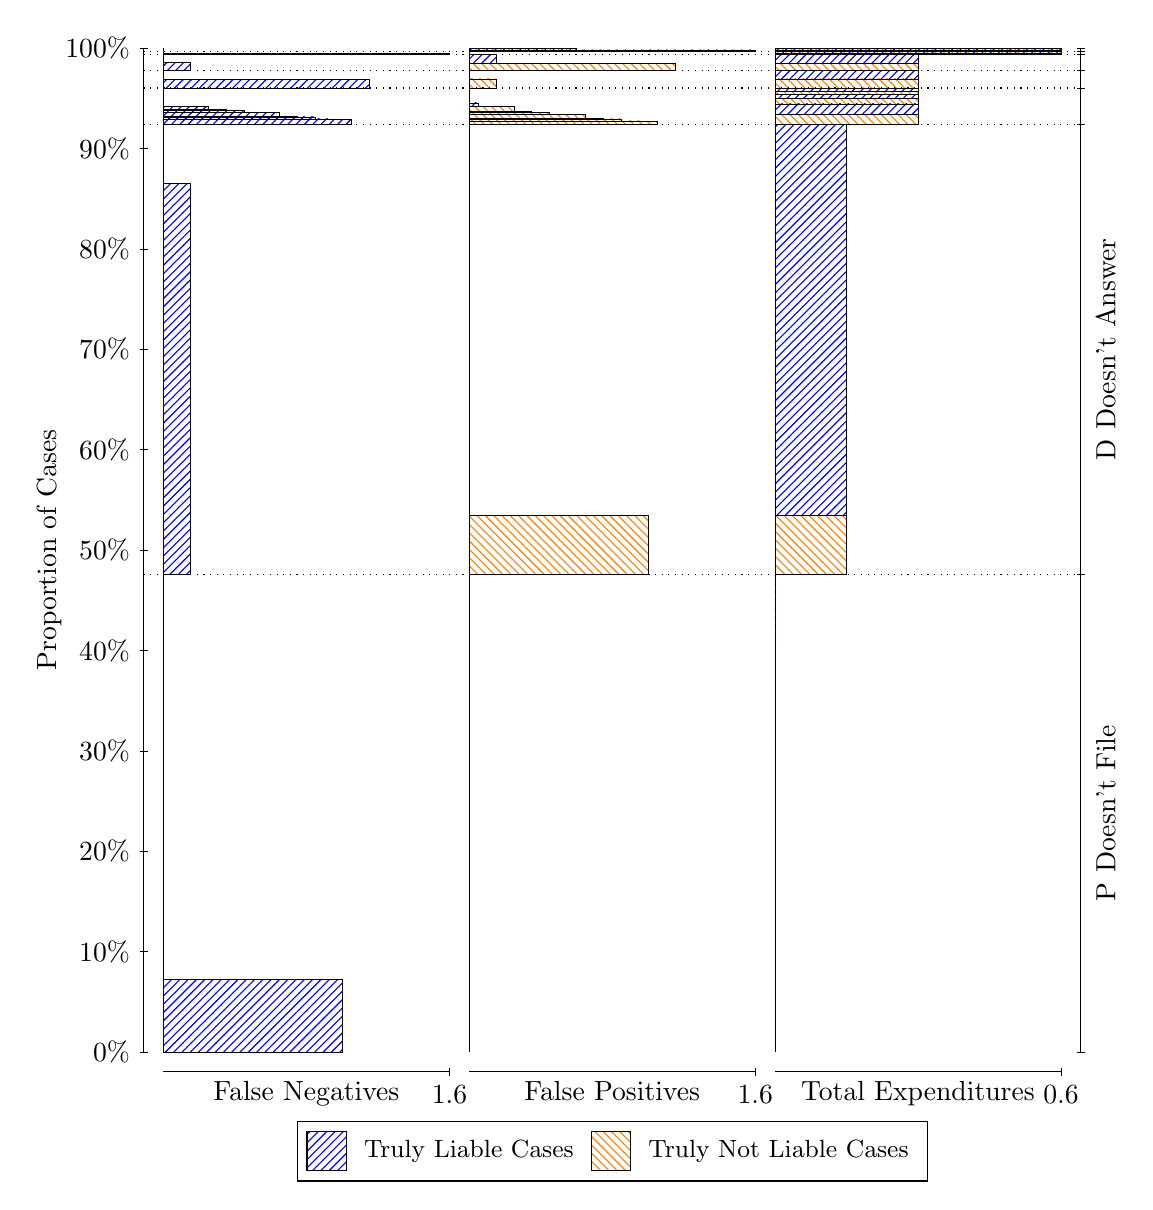
\begin{tikzpicture}
\draw[black, very thin] (1.5,1.75) -- (1.5,14.5);
\node[rotate=90, anchor=center] at (0.3, 8.125) {Proportion of Cases};
\draw[black, very thin] (1.45,1.75) -- (1.55,1.75);
\node[anchor=east] at (1.45, 1.75) {0\%};
\draw[black, very thin] (1.45,3.025) -- (1.55,3.025);
\node[anchor=east] at (1.45, 3.025) {10\%};
\draw[black, very thin] (1.45,4.3) -- (1.55,4.3);
\node[anchor=east] at (1.45, 4.3) {20\%};
\draw[black, very thin] (1.45,5.575) -- (1.55,5.575);
\node[anchor=east] at (1.45, 5.575) {30\%};
\draw[black, very thin] (1.45,6.85) -- (1.55,6.85);
\node[anchor=east] at (1.45, 6.85) {40\%};
\draw[black, very thin] (1.45,8.125) -- (1.55,8.125);
\node[anchor=east] at (1.45, 8.125) {50\%};
\draw[black, very thin] (1.45,9.4) -- (1.55,9.4);
\node[anchor=east] at (1.45, 9.4) {60\%};
\draw[black, very thin] (1.45,10.675) -- (1.55,10.675);
\node[anchor=east] at (1.45, 10.675) {70\%};
\draw[black, very thin] (1.45,11.95) -- (1.55,11.95);
\node[anchor=east] at (1.45, 11.95) {80\%};
\draw[black, very thin] (1.45,13.225) -- (1.55,13.225);
\node[anchor=east] at (1.45, 13.225) {90\%};
\draw[black, very thin] (1.45,14.5) -- (1.55,14.5);
\node[anchor=east] at (1.45, 14.5) {100\%};

\draw[black, very thin] (13.4,1.75) -- (13.4,14.5);
\draw[black, very thin] (13.35,1.75) -- (13.45,1.75);
\node[anchor=west] at (13.35, 1.75) {};
\draw[black, very thin] (13.35,7.8175) -- (13.45,7.8175);
\node[anchor=west] at (13.35, 7.8175) {};
\draw[black, very thin] (13.35,13.53) -- (13.45,13.53);
\node[anchor=west] at (13.35, 13.53) {};
\draw[black, very thin] (13.35,13.992) -- (13.45,13.992);
\node[anchor=west] at (13.35, 13.992) {};
\draw[black, very thin] (13.35,14.213) -- (13.45,14.213);
\node[anchor=west] at (13.35, 14.213) {};
\draw[black, very thin] (13.35,14.415) -- (13.45,14.415);
\node[anchor=west] at (13.35, 14.415) {};
\draw[black, very thin] (13.35,14.456) -- (13.45,14.456);
\node[anchor=west] at (13.35, 14.456) {};
\draw[black, very thin] (13.35,14.5) -- (13.45,14.5);
\node[anchor=west] at (13.35, 14.5) {};

\draw[black, very thin, pattern color=blue, pattern=north east lines] (1.75,1.75) rectangle (4.0208,2.6742);
\draw[black, very thin, pattern color=orange, pattern=north west lines] (1.75,2.6742) rectangle (1.75,7.8175);
\draw[black, very thin, pattern color=blue, pattern=north east lines] (1.75,7.8175) rectangle (2.0906,12.783);
\draw[black, very thin, pattern color=orange, pattern=north west lines] (1.75,12.783) rectangle (1.75,13.53);
\draw[black, very thin, pattern color=blue, pattern=north east lines] (1.75,13.53) rectangle (4.1344,13.589);
\draw[black, very thin, pattern color=blue, pattern=north east lines] (1.75,13.589) rectangle (3.9073,13.6);
\draw[black, very thin, pattern color=blue, pattern=north east lines] (1.75,13.6) rectangle (3.6802,13.625);
\draw[black, very thin, pattern color=blue, pattern=north east lines] (1.75,13.625) rectangle (3.4531,13.631);
\draw[black, very thin, pattern color=blue, pattern=north east lines] (1.75,13.631) rectangle (3.226,13.679);
\draw[black, very thin, pattern color=blue, pattern=north east lines] (1.75,13.679) rectangle (2.999,13.686);
\draw[black, very thin, pattern color=blue, pattern=north east lines] (1.75,13.686) rectangle (2.7719,13.711);
\draw[black, very thin, pattern color=blue, pattern=north east lines] (1.75,13.711) rectangle (2.5448,13.72);
\draw[black, very thin, pattern color=blue, pattern=north east lines] (1.75,13.72) rectangle (2.3177,13.761);
\draw[black, very thin, pattern color=orange, pattern=north west lines] (1.75,13.761) rectangle (1.75,13.992);
\draw[black, very thin, pattern color=blue, pattern=north east lines] (1.75,13.992) rectangle (4.3615,14.097);
\draw[black, very thin, pattern color=orange, pattern=north west lines] (1.75,14.097) rectangle (1.75,14.213);
\draw[black, very thin, pattern color=blue, pattern=north east lines] (1.75,14.213) rectangle (2.0906,14.32);
\draw[black, very thin, pattern color=orange, pattern=north west lines] (1.75,14.32) rectangle (1.75,14.415);
\draw[black, very thin, pattern color=blue, pattern=north east lines] (1.75,14.415) rectangle (5.3833,14.433);
\draw[black, very thin, pattern color=orange, pattern=north west lines] (1.75,14.433) rectangle (1.75,14.456);
\draw[black, very thin, pattern color=orange, pattern=north west lines] (1.75,14.456) rectangle (1.75,14.475);
\draw[black, very thin, pattern color=blue, pattern=north east lines] (1.75,14.475) rectangle (1.75,14.5);
\draw[black, very thin, pattern color=orange, pattern=north west lines] (5.6333,1.75) rectangle (5.6333,6.8933);
\draw[black, very thin, pattern color=blue, pattern=north east lines] (5.6333,6.8933) rectangle (5.6333,7.8175);
\draw[black, very thin, pattern color=orange, pattern=north west lines] (5.6333,7.8175) rectangle (7.9042,8.5647);
\draw[black, very thin, pattern color=blue, pattern=north east lines] (5.6333,8.5647) rectangle (5.6333,13.53);
\draw[black, very thin, pattern color=orange, pattern=north west lines] (5.6333,13.53) rectangle (8.0177,13.566);
\draw[black, very thin, pattern color=orange, pattern=north west lines] (5.6333,13.566) rectangle (7.7906,13.574);
\draw[black, very thin, pattern color=orange, pattern=north west lines] (5.6333,13.574) rectangle (7.5635,13.599);
\draw[black, very thin, pattern color=orange, pattern=north west lines] (5.6333,13.599) rectangle (7.3365,13.606);
\draw[black, very thin, pattern color=orange, pattern=north west lines] (5.6333,13.606) rectangle (7.1094,13.654);
\draw[black, very thin, pattern color=orange, pattern=north west lines] (5.6333,13.654) rectangle (6.8823,13.658);
\draw[black, very thin, pattern color=orange, pattern=north west lines] (5.6333,13.658) rectangle (6.8823,13.661);
\draw[black, very thin, pattern color=orange, pattern=north west lines] (5.6333,13.661) rectangle (6.6552,13.686);
\draw[black, very thin, pattern color=orange, pattern=north west lines] (5.6333,13.686) rectangle (6.4281,13.696);
\draw[black, very thin, pattern color=orange, pattern=north west lines] (5.6333,13.696) rectangle (6.201,13.762);
\draw[black, very thin, pattern color=blue, pattern=north east lines] (5.6333,13.762) rectangle (5.7469,13.802);
\draw[black, very thin, pattern color=blue, pattern=north east lines] (5.6333,13.802) rectangle (5.6333,13.992);
\draw[black, very thin, pattern color=orange, pattern=north west lines] (5.6333,13.992) rectangle (5.974,14.108);
\draw[black, very thin, pattern color=blue, pattern=north east lines] (5.6333,14.108) rectangle (5.6333,14.213);
\draw[black, very thin, pattern color=orange, pattern=north west lines] (5.6333,14.213) rectangle (8.2448,14.308);
\draw[black, very thin, pattern color=blue, pattern=north east lines] (5.6333,14.308) rectangle (5.974,14.415);
\draw[black, very thin, pattern color=orange, pattern=north west lines] (5.6333,14.415) rectangle (5.6333,14.438);
\draw[black, very thin, pattern color=blue, pattern=north east lines] (5.6333,14.438) rectangle (5.6333,14.456);
\draw[black, very thin, pattern color=orange, pattern=north west lines] (5.6333,14.456) rectangle (9.2667,14.475);
\draw[black, very thin, pattern color=blue, pattern=north east lines] (5.6333,14.475) rectangle (6.9958,14.5);
\draw[black, very thin, pattern color=orange, pattern=north west lines] (9.5167,1.75) rectangle (9.5167,6.8933);
\draw[black, very thin, pattern color=blue, pattern=north east lines] (9.5167,6.8933) rectangle (9.5167,7.8175);
\draw[black, very thin, pattern color=orange, pattern=north west lines] (9.5167,7.8175) rectangle (10.425,8.5647);
\draw[black, very thin, pattern color=blue, pattern=north east lines] (9.5167,8.5647) rectangle (10.425,13.53);
\draw[black, very thin, pattern color=orange, pattern=north west lines] (9.5167,13.53) rectangle (11.333,13.658);
\draw[black, very thin, pattern color=blue, pattern=north east lines] (9.5167,13.658) rectangle (11.333,13.791);
\draw[black, very thin, pattern color=orange, pattern=north west lines] (9.5167,13.791) rectangle (11.333,13.856);
\draw[black, very thin, pattern color=blue, pattern=north east lines] (9.5167,13.856) rectangle (11.333,13.915);
\draw[black, very thin, pattern color=orange, pattern=north west lines] (9.5167,13.915) rectangle (11.333,13.954);
\draw[black, very thin, pattern color=blue, pattern=north east lines] (9.5167,13.954) rectangle (11.333,13.992);
\draw[black, very thin, pattern color=orange, pattern=north west lines] (9.5167,13.992) rectangle (11.333,14.108);
\draw[black, very thin, pattern color=blue, pattern=north east lines] (9.5167,14.108) rectangle (11.333,14.213);
\draw[black, very thin, pattern color=orange, pattern=north west lines] (9.5167,14.213) rectangle (11.333,14.308);
\draw[black, very thin, pattern color=blue, pattern=north east lines] (9.5167,14.308) rectangle (11.333,14.415);
\draw[black, very thin, pattern color=orange, pattern=north west lines] (9.5167,14.415) rectangle (13.15,14.438);
\draw[black, very thin, pattern color=blue, pattern=north east lines] (9.5167,14.438) rectangle (13.15,14.456);
\draw[black, very thin, pattern color=orange, pattern=north west lines] (9.5167,14.456) rectangle (13.15,14.475);
\draw[black, very thin, pattern color=blue, pattern=north east lines] (9.5167,14.475) rectangle (13.15,14.5);
\draw[black, dotted] (1.5,7.8175) -- (13.4,7.8175);
\draw[black, dotted] (1.5,13.53) -- (13.4,13.53);
\draw[black, dotted] (1.5,13.992) -- (13.4,13.992);
\draw[black, dotted] (1.5,14.213) -- (13.4,14.213);
\draw[black, dotted] (1.5,14.415) -- (13.4,14.415);
\draw[black, dotted] (1.5,14.456) -- (13.4,14.456);
\draw[black, very thin] (1.75,1.5) -- (5.3833,1.5);
\node[anchor=north] at (3.5667, 1.5) {False Negatives};
\draw[black, very thin] (5.3833,1.45) -- (5.3833,1.55);
\node[anchor=north] at (5.3833, 1.45) {1.6};

\draw[black, very thin] (5.6333,1.5) -- (9.2667,1.5);
\node[anchor=north] at (7.45, 1.5) {False Positives};
\draw[black, very thin] (9.2667,1.45) -- (9.2667,1.55);
\node[anchor=north] at (9.2667, 1.45) {1.6};

\draw[black, very thin] (9.5167,1.5) -- (13.15,1.5);
\node[anchor=north] at (11.333, 1.5) {Total Expenditures};
\draw[black, very thin] (13.15,1.45) -- (13.15,1.55);
\node[anchor=north] at (13.15, 1.45) {0.6};

\node[black, centered, rotate=90] at (13.72, 4.7838) {P Doesn't File};
\node[black, centered, rotate=90] at (13.72, 10.674) {D Doesn't Answer};






\draw (7.449999999999999,1.5) node[draw=none] (baseCoordinate) {};
\begin{scope}[align=center]
        \matrix[scale=0.5, draw=black, below=0.5cm of baseCoordinate, nodes={draw}, column sep=0.1cm]{
            \node[rectangle, draw, minimum width=0.5cm, minimum height=0.5cm, pattern=north east lines, pattern color=blue] {}; &
            \node[draw=none, font=\small] (B) {Truly Liable Cases}; &
            \node[rectangle, draw, minimum width=0.5cm, minimum height=0.5cm, pattern=north west lines, pattern color=orange] {}; &
            \node[draw=none, font=\small] (B) {Truly Not Liable Cases}; \\
            };
\end{scope}

\end{tikzpicture}
\end{document}